
\documentclass[submit,techreq]{ipsj}
%\documentclass[submit,draft]{ipsj}

\usepackage{amsmath}
\usepackage{amsfonts}
\usepackage{booktabs}
\usepackage{multirow}
\usepackage[dvips]{graphicx}
\usepackage{latexsym}

\def\Underline{\setbox0\hbox\bgroup\let\\\endUnderline}
\def\endUnderline{\vphantom{y}\egroup\smash{\underline{\box0}}\\}
\def\|{\verb|}

%\setcounter{巻数}{53}
%\setcounter{号数}{10}
\setcounter{page}{1}

\受付{2011}{11}{4}
%\再受付{2011}{7}{16}   %省略可能
%\再再受付{2011}{7}{20} %省略可能
\採録{2011}{12}{1}

\begin{document}


\title{語の出現頻度と意味関係分析を用いた\\
Webからのタスク検索}

%\etitle{Subtask search}



\affiliate{KU}{京都大学大学院 情報学研究科\\
Graduate School of Informatics, Kyoto University}



\author{加藤 龍}{Ryo Kato}{KU}[r.kato@dl.kuis.kyoto-u.ac.jp]
\author{大島 裕明}{Hiroaki Ohshima}{KU}[ohshima@dl.kuis.kyoto-u.ac.jp]
\author{山本 岳洋}{Takehiro Yamamoto}{KU}[tyamamot@kuis.kyoto-u.ac.jp]
\author{加藤 誠}{Makoto P. Kato}{KU}[kato@dl.kuis.kyoto-u.ac.jp]
\author{田中 克己}{Katsumi Tanaka}{KU}[tanaka@dl.kuis.kyoto-u.ac.jp]

\begin{abstract}
本研究では,クエリとしてある目的が与えられた際に,その目的を達成するために必要なタスク集合をウェブから発見するタスク検索を提案する. 
本稿では,タスク検索の第一歩として,入力クエリを効果的にクエリ拡張することで,元のクエリでは発見不可能なタスクを含んだウェブページを収集する手法について提案する.提案手法では,検索連動型広告に着目し,動詞の出現パターンを用いてタスクに関連した動詞を抽出することで,クエリ拡張を行う. 
\end{abstract}

\begin{jkeyword}
タスク検索,検索連動型広告,クエリ拡張
\end{jkeyword}

%\begin{eabstract}
%This study is about subtask search. We propose a new method to find subtasks from the Internet. When a query is given, our method find subtasks which are needed to acomplish the task represented by the query. In our method, the system convert the query according to relationships of words such as the relationship of includingness and contradiction. The system find phrases from the pages which are listed up by our method. After that, we use language patterns which are specified in tasks to find phrases which are possible to be correct subtask.
%\end{eabstract}
%
%\begin{ekeyword}
%Task search
%\end{ekeyword}

\maketitle

%1
\section{はじめに}

ネット社会の進展に伴い,ウェブメディアには多様な情報が集積され続けている.
このようなウェブ情報をどのように探索,発見し,取捨選択するかについて,さまざまな方向からのアプローチがなされている. 
現在,多くの検索エンジンが実用化されるとともに,ウェブ情報検索やウェブ情報マイニングについて広く研究が行われている.
現行のウェブ検索エンジンは,キーワードクエリに基づく文書検索モデルに基づくものが多く,
この意味では,Webから文書ではなく情報そのものを検索するという意味でのウェブ情報検索は,いまだ多くの問題を抱えている. 
ある目的を達成する手段や方法をウェブから検索する,いわば,タスク検索も未解決の問題の一つである.

何かを成し遂げたいが,どうすれば達成できるかがわからないとき,現行のウェブ検索エンジンを使って手段・方法を見つけることが日常的にも良く行われている. 
たとえば``花粉症対策をする''をそのままクエリとして指定し,検索を実行することで,``立体マスクをつける''や``アレロック錠を飲む''というタスクを発見することができるが,検索漏れも多く,この意味で,タスク検索の再現率向上は大きな課題である.
多様なタスク(答え)が得られた段階で,初めて,安心して各タスク(方法)を比較したり,自分にとって最適な方法を考えることができるようになる.
本研究では,「目的となるタスクを達成するために,どのようなタスクがあるか」を高い再現率で発見するタスク検索手法を提案する.


タスク検索の例を説明する.たとえば``花粉症対策をする''というクエリをウェブ検索エンジンに入力すると,出力として
\begin{itemize}
\item 立体マスクをつける.
\item アレロック錠を飲む.
\item 医師の診断を受ける.
\end{itemize}

といったように,複数の異なったタスク(方法)を発見することができる.この例は,クエリのタスクに対して,検索された各々のタスク(方法)がそれ自身のみで解であり,各解は,元のタスク「花粉症対策をする」に対して,instance-ofという汎化関係が成立する.
また,同じクエリ「花粉症対策をする」に対して,次のような出力が得られる可能性もある.
\begin{itemize}
\item スギ花粉対策をする.
\item カモガヤ花粉対策をする.
\item ヒノキ花粉対策をする.
\end{itemize}
この場合は,``スギ花粉対策をする''や``ヒノキ花粉対策をする''という解は,クエリ``花粉症対策をする''というタスクに対して,a-kind-of(もしくはsubtype-of)という汎化関係が成立する.
さらに,``花粉症対策をする''というクエリに対する
出力として,以下のような項目をすべて含むページが検索されることも考えられる.
\begin{itemize}
\item 花粉症専用のマスクを販売している店を見つける.
\item その店舗で花粉症専用のマスクを購入する.
\item 隙間の無いように花粉症専用マスクを装着する.
\end{itemize}
与えられたタスク(クエリ)に対する検索解は,1つのページが1つの解に対応する場合や,複数のページ(に記載されたタスク)の集約が1つの解に対応する場合があり,現行のウェブ検索エンジンによる解ページのランキングでは不十分であることが予想される. 
花粉症対策の方法は非常に多様であり,高くランクづけされたページであっても花粉症対策の方法のごく一部を含んでいるにすぎない場合もある. 
また,高くランクづけされたページ同士は内容が重複していることが多く,高ランクのページを見て回っても,発見できる花粉症対策の方法の数は増えないことも考えられる.

このようなタスク検索が実用的なレベルに達すれば、以下に示すような,多くの応用例が考えられる.
%たとえば,以下のような応用例があげられる.
\begin{itemize}
\item 入力クエリに関連するタスクをクエリ推薦としてユーザに提示する.
\item ``マスクをつける''という入力クエリに対して,``アレロック錠を飲む''という,
ある同一の目的を達成する代替タスクをユーザに推薦する.
\item 1つのページに複数のタスクが網羅的に記載されているページの発見や,多様なタスクを含んだページ集合のランキングといった,タスクベースのページランキング.
\end{itemize}


%
%現在多くの人々がウェブ検索エンジンを利用し,日常的に情報収集を行っている.
%ウェブ検索エンジンを利用するユーザの情報要求はさまざまであるが,
%そのうちの一つとして,ある目的を達成する手段を網羅的に調べたいという情報要求があげられる.
%たとえば,花粉症を発症してしまったユーザが,花粉症の対策としてどのような方法が存在するのかを調べたり,
%禁煙を始めようとしているユーザが,どのような方法があるのか調べたりするような場合がある.
%
%こうした検索の特徴として,目的を達成するための手段が多数存在するということがあげられる.
%たとえば,``花粉症の対策をする''ことを考えた場合,``立体マスクをつける'',``アレロック錠を飲む'',
%``空気清浄機を使用する'',``レーザ治療を受ける''などはじめとして,ウェブにはさまざまな方法が記述されている.
%しかし,ウェブ検索エンジンを利用してこうした方法を網羅的に収集することを考えた場合,
%ユーザはウェブページを調べながらどのような方法が存在するのか調べながら,
%複数のクエリを用いてウェブ検索していく必要がある.
%
%
%本研究では,``花粉症の対策をする''に対する``立体マスクをつける''や``アレロック錠を飲む''といった,
%入力となる目的を一部あるいは全て達成するような行動を``サブタスク''と定義し(詳しくは\ref{sec:task}章で述べる),
%こうしたサブタスクをウェブから網羅的に発見する研究に取り組む.
%このような,ある入力となる目的を達成するためのサブタスクが網羅的に発見できると,多くのアプリケーションが考えられる.
%たとえば,以下のような応用例があげられる.
%\begin{itemize}
%\item 入力クエリに関連するサブタスクをクエリ推薦のように提示する(\figref{fig:future_app}).
%\item 「立体マスクをつける」のような入力クエリに対して,「鼻炎薬を飲む」のような,ある同一の目的を達成するような代替手段をユーザに推薦する.
%\item より多くのサブタスクを含み,かつ多くのサブタスクが網羅されているようなウェブページ集合を上位にランキングすることで,タスクベースの文書ランキングを行う.
%\end{itemize}


%\begin{figure}[tb]
%\centering
%\includegraphics[width=0.7\hsize]{application.eps}
%\vspace{-1em}
%\caption{タスク検索のアプリケーション例}
%\ecaption{Application of Task Search.}
%\label{fig:future_app}
%\end{figure}

このようなタスク検索を実現するための第一歩として,本研究では,
入力となるクエリを達成するためのタスクを含んだウェブページを網羅的に集めるための手法を提案する.
提案手法では検索連動型広告に着目し,入力クエリに関連した動詞を自動的に抽出し,入力クエリを拡張することで,
入力クエリ単体では得ることができないタスクをより多く発見する手法を提案し,その有効性を検証する.

本稿の構成は以下のとおりである.
まず,2章で関連研究を紹介する.
3章では,本研究で扱うタスクとサブタスクの概念を定義するとともに,
その関係性を整理する.
4章で提案手法について説明し,5章で評価実験について述べた後,
最後に本稿をまとめる.


%\begin{itemize}
%\item \|立体マスクをつける|
%\item \|アレロック錠を飲む|
%\item \|医師の診断を受ける|
%\item \|植物に近寄らない|
%\end{itemize}


%といったように,複数の異なった選択肢を複数発見する.これがサブタスク検索の例である. このように,できるだけ多くの手法を探そうとする検索は現在の一般的な検索エンジンでは困難である. 花粉症対策の方法は非常に多様であり,高くランクづけされたページであっても花粉症対策の方法のごく一部を含んでいるにすぎない. また高くランクづけされたページ同士は内容が重複していることが多く,高ランクのページを見て回っても,発見できる花粉症対策の方法の数は増えない。
%
%このようなサブタスク検索が実用的なレベルに達すれば、\figref{fig:future_app}のように、 現在の検索エンジンが実装しているサジェスト機能にサブタスク検索を組み込むといった応用が考えられる。

%
%
%
%誕生以来,Webには多様な資料が集積され続けている. 情報をどう走査,発見し,取捨選択するか,様々な方向からのアプローチがなされている. 
%現在,いくつもの検索エンジンが実用化され,Webを舞台に情報発見や集約を行っている. だが,Webにおける情報検索は,いまだ多くの問題を抱えている. 
%そのうちの一つとして,目的を達成する手段を発見したいとき,できるだけ多くの方法を探そうとしても意外と見つけられないことがあげられる.
%
%
%なにかを成し遂げたいが,どうすれば成功するかわからないとき,Web検索を使って実現方法を考える行為がよく行われている. たとえば「花粉症対策をする方法」をクエリに検索することで,立体マスクをつける」や「アレロック錠を飲む」を発見することができる. だが,そうして発見できた「花粉対策をする方法」を採用すべきなのか,簡単にはわからない. まだ発見できていない「花粉対策をする方法」のほうがよいかもしれないからだ。
%
%
%こうした状況では,多くのユーザーは「タスクを遂行するためにどんな方法があるか」をできるだけ多く発見するサブタスク検索を求める. 多様な答えが得られた段階で,初めて,安心して各方法を比較したり,自分にとって最適な方法を考えることができるようになる.
%
%
%サブタスク検索の例を説明する.たとえば「花粉症対策をする」というクエリを入力すると,出力として
%
%
%
%
%サブタスク検索は、タスクを遂行する方法が複数あり、どれがベストかわからない状態で役割を果たす。\figref{fig:future_app}は、まさしくその一例である。クエリに「iPhone ゲーム 開発」と入力した結果、通常のWeb検索であってもiPhoneゲームの作り方についてのWebページを非常に多量に発見できる。しかし、通常の検索のみでは人気の高いページだけが上位にランクづけされてしまう。そのため、iPhoneのゲームを開発するためにやるべき行動をすべて網羅できない。このとき、「App storeの審査を受ける」といった、やらねばならないことだが、上位ページではあまり言及されないタスクに気づかない、といった問題が発生しうる。こうした状況でサブタスク検索を行うことで、iPhoneのゲームを開発するために必要なタスクがすべて明らかになり、タスク遂行のためのロードマップを描きやすくなる。
%
%逆にサブタスク検索が不得意なこととして、遂行する方法がひとつのタスクがある。たとえばすでに手元に本があるとき「手元の本を読む」というタスクを遂行する方法はひとつである。
%
%サブタスク検索が有効に働くのは、多くの、時間のかかる作業をせねばならないときである。
%
%
%タスク検索は、Web検索のなかでもかなりの割合を占めている。サブタスク検索を実現することは、Webでの検索体験を向上させる点で非常に有意義である。
%
%以下、本稿では可能な限り多様な方法をWebから発見する手法を提案し,評価する。


%1.1
\section{関連研究}
\subsection{タスク検索}
1章で述べたような,ユーザのタスクに基づく検索の支援を目的とした研究は,近年注目を集めはじめている.
たとえば,Yamamotoらは,\textit{search goal}と\textit{subgoal}という概念を提案し,
検索連動型広告(スポンサードサーチ)のログを利用し,入力クエリに関連したsubgoalを関連クエリのクラスタリングにより発見する手法を提案している\cite{yamamoto2012wisdom}.
彼らの定義によれば,search goalとは``ユーザが達成したいと考えている行動''であり,
あるsearch goal $x$を達成することで別のsearch goal $y$の一部あるいは全てを達成するとき,
xはyのsubgoalである,と定義している.
我々が提案するタスク検索は,タスク間の階層的な関係を考えている点でYamamotoらのsearch goalとsubgoalの関係に近い.
しかし,本稿ではタスクを行動だけではなくユーザの状態の遷移という点から捉え,
より詳細にタスクをモデル化している(詳しくは\ref{sec:task}章で述べる).

また,Hassanらも,ユーザのタスクを達成するための支援を行うための手法を提案している\cite{hassan2012task}.
彼らは,あるウェブページに関するOpen Directory Project(ODP)から得られるカテゴリを1つのタスクとして捉え,
検索ログから関連するタスク集合を抽出することで,あるクエリに関連したタスク集合を自動的に発見する手法を提案している.
ほかにも,湯本らは手順情報に着目し,ハウツー的な文書から手順情報を抽出し構造化する手法を提案している\cite{yumotoHowTo}.
こうした,ある目的を達成するために必要な手順情報を発見することも我々が扱うタスク検索の一種であると捉えることができる.


\subsection{検索連動型広告を利用したクエリ変換}
\label{sec:tamugi}
検索連動型広告を対象とした研究の多くは,広告の検索精度の向上\cite{BroderAdQueryExpansion}やクリックスルーレートの予測\cite{RichardsonEstimatingCTR},
検索連動型広告におけるユーザの検索行為の分析\cite{jansen2005examining}\cite{DanescuNiculescuMizilInterplayAd}などが主である.


こうした研究に対し,本稿では検索連動型広告に着目し,タスクを含んだウェブページを得るためのクエリ修正を行う.
検索連動型広告に着目した同様の研究として,田麥らの研究がある\cite{tamugiDEIM}\cite{tamugiDBS}\cite{tamugiMS}.
田麥らは,ギターの買い取りやホテルの予約といった,
さまざまなサービスを提供しているウェブページを効率的に発見する手法について取り組んでいる.
彼らは,``中古ギターを売りたい''という情報要求を持ったユーザの場合,``中古ギター 売却''というクエリでウェブ検索を行うよりも,``中古ギター 買取''というように,中古ギターの買い取り業者というサービス提供者側の視点に立ったクエリに変換してウェブ検索する方が,目的のサービスに関するページを得やすいと指摘している.
彼らは,``売却''に対する``買取''のようなクエリの変換ルールとして,以下の6パターンを提案している.
\begin{enumerate}
\item \textbf{語の逆意関係:} ``中古ギター 売却''に対する``中古ギター 買取''のような,動作の主体の違いにより動詞の意味が逆転する動詞.
\item \textbf{語の同義関係:} ``荷物 送る''に対する``荷物 配送''のような,同義語の関係にある単語.
\item \textbf{語の併立関係:} ``部屋 借りる''に対する``部屋 探す''のような,動作の併立(entailment)関係にある動詞.
\item \textbf{語の兄弟語関係:} ``ぬいぐるみ 処分''に対する``ぬいぐるみ 供養''のような,同一の結果をもたらすが異なる意味の動詞.
\item \textbf{タスクの価値を表す語:} 
``ブランド品 売却''に対する``ブランド品 売却 高価''のような,タスクの価値を宣伝するような語.
\item \textbf{タスク提供者が提供する語:} ``ダンス 習う''に対する``ダンス 学校''のような,タスクの提供者側と関連した語.
\end{enumerate}
彼らの研究では,入力クエリとそれに関連した検索連動型広告から,上記ルールに基づいて,変換すべきクエリを抽出し,
それをクエリ拡張に用いることで,サービスを提供するウェブページに関する検索の適合率および再現率が向上できることを示している.

%%%%%%%%%%%%%%%%%%%%%%%%%%%%%%%%%
\section{タスクとタスク検索}
\label{sec:task}

本章では,我々が取り組むタスク検索の検索モデルについて説明する.
1章で述べたように,ある入力タスクと,それを達成することに関わるタスクには,
instance-of関係やsubtype-of関係,part-of関係など多様な関係が存在する.
タスク検索を行うためには,まずこうした多様なタスク間の関係をモデル化する必要がある.


\subsection{行動と状態に基づくタスクのモデル化}
本稿では,行動と状態という2つの概念を用いてタスクをモデル化する.
\figref{fig:state_action}は,``花粉症の対策をする''ということを
\textit{行動}と\textit{状態}でモデル化した図であり,
2つの状態と1つの行動で表現されている.
図中の2つの状態のうち,左側の``花粉症の対策をしていない状態''は,
タスクを実行する前の状態であり,右側の``花粉症の対策をした状態''は,
タスク実行後の,目標とする状態を表している.
それらの状態間を遷移させるものが行動であり,
ここでは``花粉症の対策をする''という行動があることを表している.
このように,タスクというものを考慮するにあたって,
状態とその状態間を遷移する行動が重要な要因となると我々は考えている.

状態と行動という2つの概念に基づき,本研究ではタスクを,
\textbf{ある初期状態から目的とする状態への遷移を可能とする,一連の行動}
,と定義する.





ここで,行動と状態という2種類の概念を用いて,``花粉症の対策をした状態''という
目標を達成するためのタスクについて考えてみる.
その候補として,たとえば,``マスクをつける'',``アレロック錠を飲む'',``スギ花粉対策をする''と
いった3つのタスクが考えられる.
これら3つのタスクは,全て与えられた目標を達成するものであると考えられ,
\textit{状態}と\textit{行動}のモデルに当てはめて考えると,\figref{fig:parallel}のようになる.
ここでの考え方は,目標となる``花粉症の対策をした状態''は,``マスクをした状態'',``アレロック錠を飲んだ状態'',``スギ花粉対策をした状態''といった,花粉症対策に関連したさまざまな状態の集合であると捉えている.
このように考えることで,``花粉''と``スギ花粉''のようなsubtype-of関係の
扱いと,``花粉''と``マスク''という概念構造的には階層関係が
存在しない関係を,同様に扱うことが可能となる.


\begin{figure}[t]
\centering
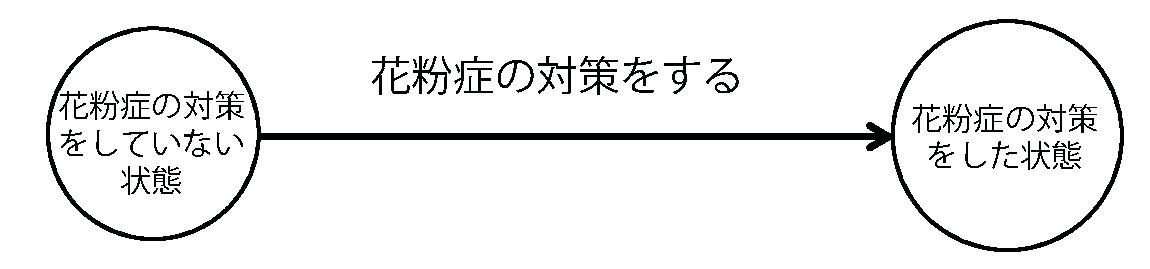
\includegraphics[width=0.9\hsize]{state_action.eps}
\vspace{-0.5em}
\caption{``花粉症の対策''に関する状態と行動の例}
\ecaption{States and its action for ``treat pollen allergy.''}
\label{fig:state_action}
\end{figure}


\begin{figure}[t]
\centering
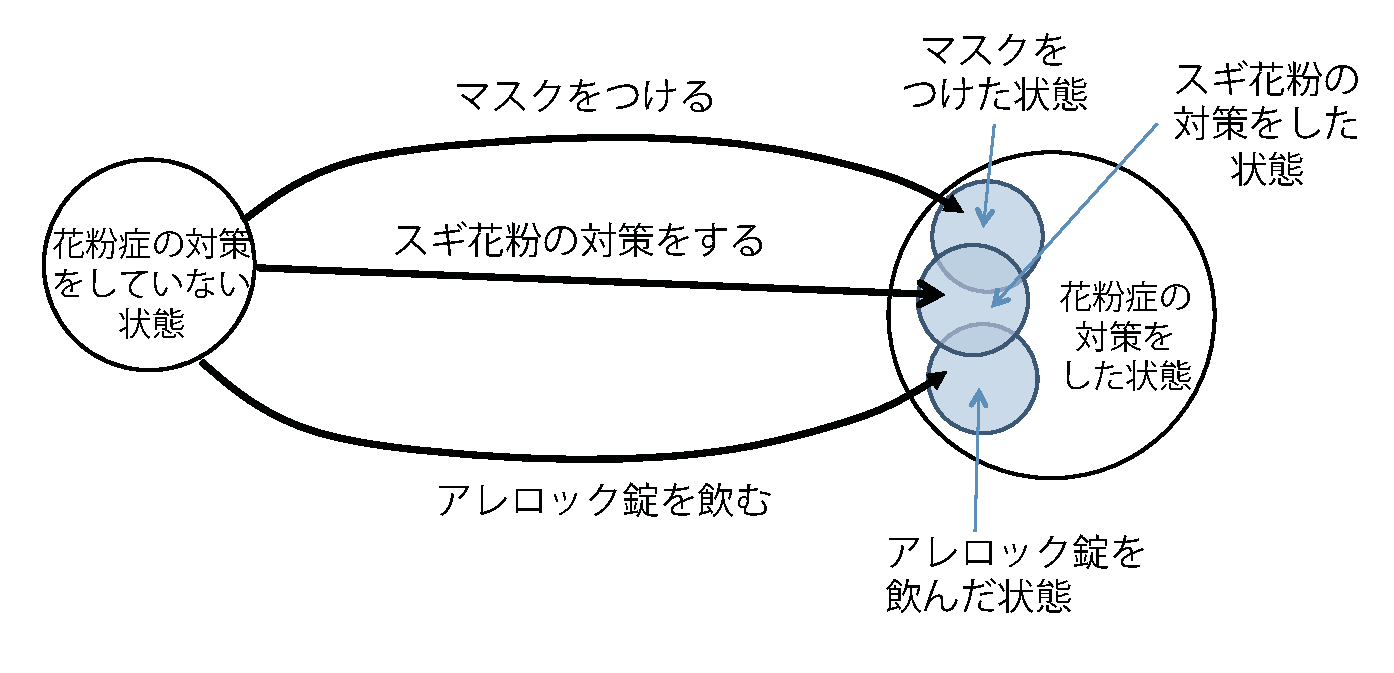
\includegraphics[width=0.9\hsize]{parallel.eps}
\vspace{-0.5em}
\caption{``花粉症の対策をした状態''になるための複数の行動の例}
\ecaption{Example actions for achieving  ``treat pollen allergy.''}
\label{fig:parallel}
\end{figure}



\begin{figure}[t]
\centering
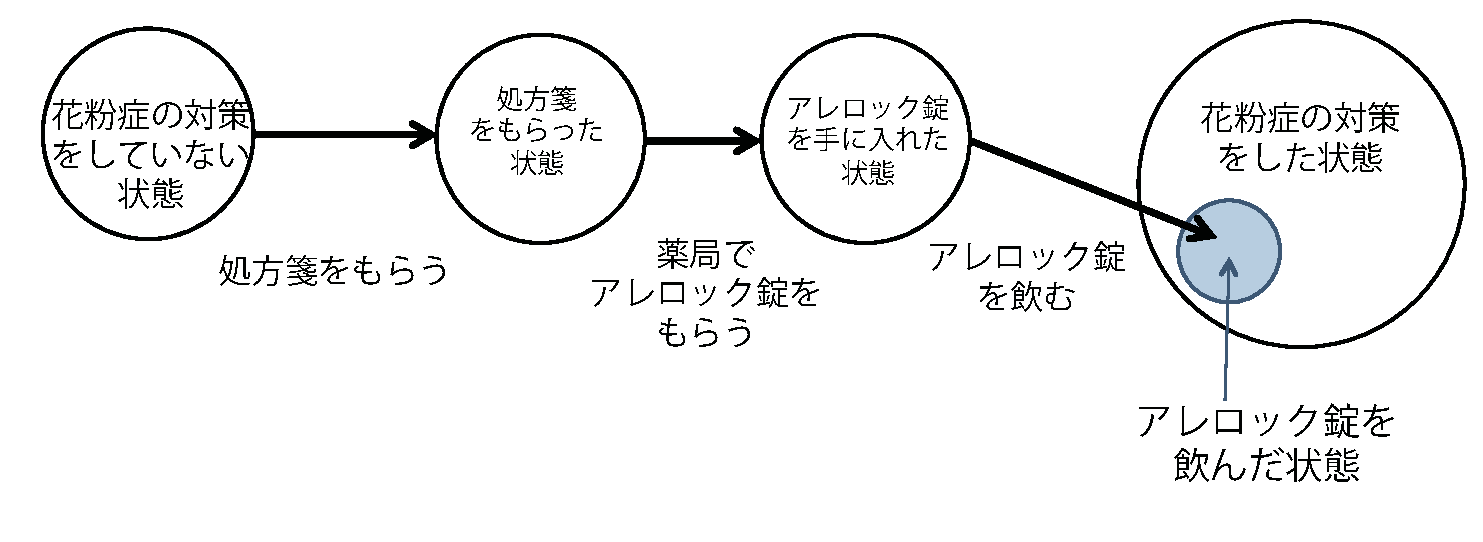
\includegraphics[width=0.9\hsize]{sequence.eps}
\vspace{-0.5em}
\caption{複数の行動からなるタスクの例}
\ecaption{Example task achieved by multiple states and actions.}
\label{fig:sequence}
\end{figure}

このモデルにおいて,行動は,一般に,複数の行動に分割することが可能である.
行動と行動の間には,中間状態が存在することになる.
たとえば,``アレロック錠を飲む''という花粉症の対策は,
まず病院に行って処方箋をもらい,その後薬局でアレロック錠をもらい,そしてアレロック錠を飲むという,複数の行動のシーケンスととらえることができる.
中間状態としては,``処方箋をもらった状態''や``アレロック錠を手に入れた状態''などが
考えられる.
これを,状態と行動のモデルで表現すると\figref{fig:sequence}のようになる.


%ここで,より厳密に上記のタスクを定義することを考える.
%いま,取り得る全てのアトミックな状態があるとし,その集合を${\cal A}$とし,
%そのべき集合を$2^{\cal {A}}$とする.
%また,ある状態から別の状態へ遷移する際にユーザが取るべき動作を{\textbf 行動}とすると,
%行動は状態と状態の直積$2^{\cal A} \times 2^{\cal A}$で表現することができる.

%
%このとき,タスクとはある初期状態$S_{0} \in 2^{\cal {A}}$,目的の状態$S \in 2^{\cal {A}}$へ遷移するための行動$V \in {\cal A} \times {\cal A}$であると定義することができる. 



\subsection{タスク検索}
ここまでの議論を踏まえて,タスク検索について定義する.

まず,ユーザより入力として与えられるのは,Web検索エンジンに入力されるような
クエリ文字列である.
本稿におけるタスク検索とは,入力として与えられたクエリ文字列が明示的,または,
非明示的に示す目標の状態への遷移を実現する行動の集合を発見することと定義する.
たとえば,``花粉症  対策''という入力クエリに対して,
``マスクをつける'',``スギ花粉対策をする'',``アレロック錠を飲む'',``処方箋をもらう''といった行動が求める出力となる.



%%%%%%%%%%%%%%%%%%%%%%%%%%%%%%%%%%%%%%%%%%%%%
%%%%%%%%%%%%%%%%%%%%%%%%%%%%%%%%%%%%%%%%%%%%%
\section{検索連動型広告を用いたクエリ拡張に基づくタスクを含むウェブページの発見}
\label{sec:method}
本稿では,3章で述べたタスク検索を実現するための第一歩として,
タスクを含むウェブページを網羅的に発見するための手法を提案する.
1章でも述べたとおり,通常のウェブ検索を行っただけでは,ある目的を達成するためのタスクを網羅的に収集することは難しい.
そこで,本稿では,検索エンジンの検索連動型広告に着目し,そこからタスクに関連した動詞を用いて入力クエリを拡張することで,
元の入力クエリから得られるウェブページには含まれていないようなタスクを含んだウェブページを発見する.


\subsection{検索連動型広告を用いたクエリ拡張}
前章で説明したように,タスクとは,目的を達成するために必要な,ユーザが取るべき行動と考えることができる.
Yamamotoらや田麥らは,そうしたタスクは検索エンジンの検索連動型広告と非常に関連が深いことを指摘している.
現在,多くの商用検索エンジンでは,ユーザが入力したクエリに対して,
広告主によって登録された広告のうち関連度の高いものが,検索結果ページ上に表示されるようになっている.
この検索連動型広告とタスク検索の関係に関して,
たとえば,Yamamotoらは,タスク検索は一般的に達成することが困難であるため,そのようなドメインに多くの広告が登録されており,
1つ1つの広告は特定の行動やトランザクションに関連していると述べている\cite{yamamoto2012wisdom}.
また,田麥らは,あるサービスを検索する場合,その多くは検索連動型広告に出現しており,
検索連動型広告を利用することでサービスに関するウェブを効率的に検索できることを示している\cite{tamugiDEIM}.

そこで,本稿ではクエリ拡張を行う際の拡張語を選択するための情報源として,
検索連動型広告を利用する.
検索連動型広告を利用することで,タスクに関連し,かつ通常のウェブ検索結果からでは得られないようなタスクに関連した
語句がクエリ拡張語として得られることが期待される.

%本稿ではスポンサードサーチを用いたサブタスク検索を提案する。スポンサードサーチとは、ユーザーの入力した検索クエリに対応した広告を表示するシステムである。GoogleやBing, Yahoo!など、多くのサーチエンジンがスポンサードサーチを提供している。スポンサードサーチによりユーザーは自分の入力したクエリに適した広告ページを見ることができ、広告主は広告の商品に適したユーザーにアプローチすることができる。
%
%
%スポンサードサーチに着目した理由を述べる。スポンサードサーチには、商品を購買しそうなユーザーの目に留まるように多くの工夫がなされている。具体的には、商品に対応したクエリを入力したときに広告が表示されるように設定されており、スニペットの文章は商品のニーズを端的に表現している。これは\cite{yamatake}が指摘した通りである。このような特徴を利用すれば、サブタスク検索に使えると我々は考えている。
%
%ユーザーが目的とするゴールに到達するために、スポンサードサーチに広告を出している企業の商品を使うことは有効な場合が多い。本稿の\ref{sec:evaluate}で用いた「花粉症対策をする」といったクエリであれば、「立体マスクをつける」「花粉症の薬を飲む」といったサブタスクはどちらも商品を使用することで達成できる。
%
%また実際に商品そのものを使わなくとも、何らかの手段で商品の効能が発揮された状態になれば、目的が達成されることも多い。「花粉をシャットダウンする」という広告スニペットから「花粉をシャットダウンすることが花粉症対策のサブタスクである」と推論することができる。



%3.2
\subsection{手法の流れ}
\label{sec:flow}
提案手法の概要を\figref{fig:overview_method2}に示す.
本手法は以下の流れでウェブページを取得する.

\begin{figure}[t]
\centering
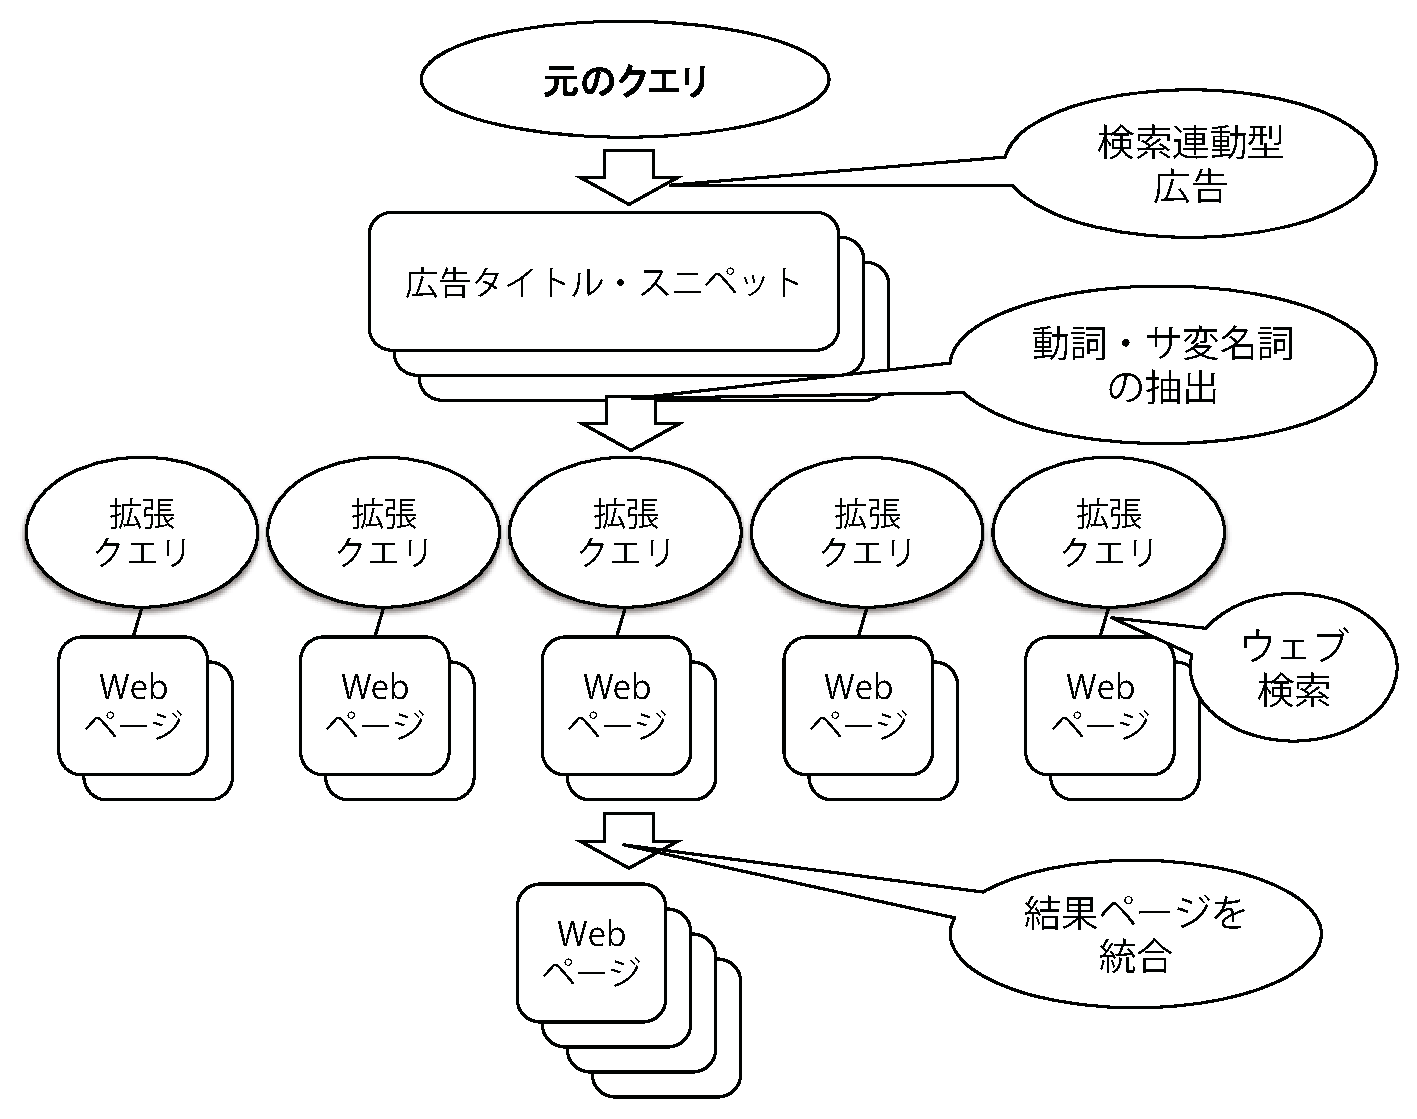
\includegraphics[width=0.75\hsize]{method.eps}
\caption{提案手法の概要}
\ecaption{Overview of our method.}
\label{fig:overview_method2}
\vspace{-2em}
\end{figure}


\begin{enumerate}
\item タスク(目的となる状態)を表したクエリ$q$を受け取る.
\item $q_{0}$でウェブ検索を行い,$n$件の検索連動型広告$\{ a_{1}, \ldots, a_{n} \}$を取得する.
\item $\{ a_{1} \ldots a_{n} \}$のタイトルおよびスニペットに対して形態素解析を行い,出現する動詞およびサ変接続名詞を抽出し出現回数を計算する(得られた単語集合を$W$,単語$w \in W$の出現回数を${\rm tf}_{w}$とする).
\item ${\rm tf}_{w}$の高い単語上位$m$件($\{ w'_{1} \ldots w'_{m} \}$とする)を取得する.
\item ウェブページ集合を$D = \phi$とし, (4)で得られたそれぞれの単語 $w_{i}$($1 \leq i \leq m$)について,$|D|=k$となるまで以下のプロセスを繰り返す.
\begin{enumerate}
\item 元のクエリに得られた単語を追加したクエリ$q_{i} = q \wedge w_{i}$を作成する.
\item 得られたクエリ$q_{i}$でウェブ検索を行い,上位$k'$件のウェブページ$\{ d_{1}^{(i)} \ldots d_{k'}^{(i)} \}$を取得する.
\item 得られたウェブページを$d_{1}^{(i)}$から順に$D$に追加($D \leftarrow D \cup \{ d_{1}^{k'} \}$)する.
このとき,$|D| = k$となればステップ(6)へ移行する.
\end{enumerate}
\item 得られたウェブページ集合$D$を返す.
\end{enumerate}


上記の手法を適用することで,元のクエリ$q$で得られるウェブページ集合より多くのタスクを含んだ,
つまり得られるタスクという観点で再現率の高いウェブページ集合を集めることができると考えられる.




%4
\section{評価実験}
\label{sec:evaluate}

本章では,\ref{sec:method}章で提案したクエリ拡張手法が,
元の入力クエリで得られた上位$k$件のウェブページから得られるタスクに対して,
どの程度新しいタスクを含んだウェブページを発見できているのかを評価した.

\subsection{ベースライン手法と実験設定}
提案手法の有効性を検証するため,検索連動型広告を用いず,
通常のウェブ検索の検索結果を用いてクエリ拡張を行いウェブページを収集する手法をベースライン手法として用意した.
具体的には,\ref{sec:flow}節で示した手法のうち,$\{a_{1}, \ldots, a_{n} \}$を検索連動型広告ではなく,通常のウェブ検索結果上位$n$件とした手法である.

実験にあたりウェブ検索結果の取得にはGoogle Custom Search API\footnote{https://developers.google.com/custom-search/?hl=ja}を用い,
検索連動型広告の取得には,Yahoo! Japanが提供するスポンサードサーチ\footnote{http://search.yahoo.co.jp/search/ss}を利用した.
また,形態素解析にはMeCab\footnote{https://code.google.com/p/mecab/}を用いた.

\label{sec:flow}節で述べた手法のパラメータについては,今回の実験では,$n=15$,$k=20$,$k'=5$と設定した.
すなわち,クエリ拡張を行い最終的に20件のウェブページを取得し,
そのウェブページにどの程度,元のクエリで得られる20件のウェブページに含まれていないタスクが含まれているのかを評価した.


%4.1.3
\subsubsection{実験に用いたクエリ}

本稿では,``花粉症の対策をする'',``部屋を掃除する'',``結婚する'',
``コーヒーを淹れる'',``ダイエットする''という
5種類のクエリを用いて実験を行った.
これらのクエリを選択した理由は,これらの目的を達成する手段が豊富に存在すると考えたためである.

\subsection{評価尺度}
提案手法の性能を評価するに当たって,以下の2種類の評価基準を設け,
人手による検証を行った.

\begin{itemize}
\item \textbf{行動数:}クエリ拡張で得られた上位20件のウェブページ集合から得られた,目的の達成に必要な行動の数のうち,元のクエリで検索して得られた上位20件のウェブページには存在しなかった行動の数.
\item \textbf{詳細度:}新しく得られた行動のうち,その行動を達成するために必要な情報が得られたウェブページに書かれている場合はその行動に対して2点,行動が列挙されているだけでその行動に達成するために必要な情報が得られない場合は1点として上記の行動数を重みづけた尺度.
\end{itemize}

たとえば,クエリ拡張を行い新しく取得したウェブページの中から,``加湿器を使う''という行動が得られたとき,
行動数を1として計算する.
その際,もしウェブページに加湿器を購入するための情報や良い加湿器に関する情報などが含まれていたら詳細度を2点,そうでない場合は1点として計算する.



%%%%%%%%%%%%%
\subsection{実験結果}
\label{sec:result}
得られた結果を\tabref{tbl:super_sub}に示す.
まず,新しく得られた行動数に着目してみると,\tabref{tbl:super_sub}から分かるように,``部屋の掃除をする'',``結婚式する'',``コーヒーを淹れる''というクエリでは,
目的を達成するために必要な行動として,提案手法によりクエリ拡張を行うことで新しいものがベースラインよりも多く取得できていることが分かる.
また,詳細度について着目してみると,\tabref{tbl:super_sub}から分かるように,``ダイエットをする''以外の4つのクエリについて,提案手法がベースライン手法を上回っていることが分かる.
これは,検索連動型広告を用いてクエリ拡張を行うことで,よりタスクの達成に特化した,タスクの達成に必要な情報が記載されたウェブページが取得できたことを示していると考えられる.

クエリ拡張語としてどのようなものが得られていたのかを分析すると,
``部屋の掃除をする''というクエリについては,提案手法では``クリーニング'',``配送'',``洗浄''といた単語が得られていた.
一方ベースラインでは,``上がる''や``維持''といった単語が得られており,検索連動型広告を利用することで,
タスクに関連した単語がクエリ拡張語として得られていることが分かる.
また,``部屋の掃除をする''というクエリでは,提案手法は``掃除の代行業者に頼む''というタスクを含んだウェブページが得られており,
検索連動型広告に出現するクリーニングや洗浄といった単語が,こうしたタスクに関連したウェブページの発見を可能にしたと考えられる.


一方で,``ダイエットする''というクエリについては,どちらの評価尺度ともベースラインと比較して,高い値は得られなかった.
提案手法では,``ダイエットをする''に対して,``吸引'',``体験''といった単語が拡張語として得られており,実際に``吸引''という語を追加することで脂肪吸引に関するウェブページを発見することができていた.
一方で,ベースライン手法では``食べる''という語がクエリ拡張語として得られており,
元のクエリでは既にダイエットに有効な食事に関するウェブページが多く出現していたものの,
``食べる''を元のクエリに追加することで,より多様な食事に関するダイエット方法を記載したページが得られ,
結果として提案手法よりも得られる行動数が多くなっていた.


\begin{table}[t] 
\caption{クエリ拡張により新しく得られた行動の数と詳細度.提案手法がベースラインよりも高い値を示した評価尺度については太字で表示している} 
\ecaption{Number of obtained actions and their detailedness by query expansion technique.}
\label{tbl:super_sub}
\begin{center}
\begin{tabular}{l l c c c c}\toprule\toprule
 & & \multicolumn{2}{c}{提案手法} & \multicolumn{2}{c}{ベースライン} \\ \cmidrule(r){3-4} \cmidrule(r){5-6}
 & &  行動数 & 詳細度 & 行動数 & 詳細度 \\ \midrule
\multirow{5}{*}{\rotatebox{90}{\textbf{入力クエリ}}} & 花粉症の対策をする & 11 & \textbf{16} & 11 & 13 \\
 & 部屋の掃除をする & \textbf{16} & \textbf{32} & 7 & 7 \\
 & 結婚する & \textbf{10} & \textbf{20} & 3 & 6 \\
 & コーヒーを淹れる & \textbf{5} & \textbf{9} & 4 & 4 \\
 & ダイエットする & 5 & 9 & 5 & 10 \\ \bottomrule
\end{tabular}
\end{center}
\vspace{-1.0em}
\end{table}



%5
\section{考察}
\label{sec:discussion}

\subsection{クエリ拡張語のランキング}
今回提案手法で得られたクエリ拡張語の中には,\label{sec:result}節で示したように,タスクに関連した動詞が得られていることもあったが,タスクとは関連しない単語も多くクエリ拡張語として得られていた.
今回は,単純に出現頻度だけを利用してクエリ拡張語を選択したが,
将来的には\ref{sec:tamugi}節で紹介したような,タスク提供者側と利用者間の単語の意味関係に踏み込んで,
クエリ拡張に利用する語を抽出することが必要であると考えられる.

\subsection{subtype-of関係に基づく結果の分析}
3章では,目標となる状態を達成する際に,instance-of関係やsubtype-of関係にある状態を達成するようなタスクがタスク検索の検索対象であることを述べた.
そこで,クエリ拡張により新しく得られたタスクが,どの程度このような関係に関連しているのかを人手で分類した.
このとき,あるタスクが元のクエリが示すタスクのsubtype-of関係であるとは,
得られたタスクが示す名詞あるいは動詞が,元のクエリが示すタスクの名詞または動詞のsubtype-of関係となっていることとした.
たとえば,``コーヒーを淹れる''という入力クエリに対して,``アイスコーヒーを淹れる''というタスクは,``アイスコーヒー''が``コーヒー''のsubtype-of関係であるため,
``アイスコーヒーを淹れる''は``コーヒーを淹れる''のsubtype-of関係である.

\tabref{tbl:subtype}は,得られたウェブページ中に記載されていたタスクをsubtype-of関係かそうでないかに基づいて分類した結果である.
表から分かるとおり,今回得られたタスクの多くはsubtype-of関係にないタスクが得られていることが分かる.
これは,今回の手法は動詞に着目した手法であり,``コーヒー''に対する``アイスコーヒー''のような,
subtype-of関係にあるようなタスク間の関係を全く考慮していないためであると考えられる.
このような,subtype-of関係にあるようなタスクは,それ単体ではユーザの入力クエリとなる達成に役に立つ情報であるとはいえない.
しかし,subtype-of関係にあるようなタスクを発見することができれば,
それを基にそのタスクの達成に必要なタスクを再帰的に発見していくことで,
入力タスクにも適用可能なタスクが発見可能となると考えられる.
さまざまなタスクを網羅的に取得するためには,動詞のみならず,名詞の階層的関係なども考慮しながらページを取得する必要があると考えられる.

%
%\begin{table}[t] 
%\caption{``コーヒーを淹れる''とsubtype-of関係にあるようなタスク.
%表中の×印は,そのタスクがウェブページから得られたことを示している.} 
%\ecaption{Example tasks which have an subtype-of relationship between ``make coffee''}
%\label{tbl:coffee}
%\scalebox{0.85}{
%\hbox to\hsize{\hfil
%\begin{tabular}{l c c c}\toprule\toprule
% & 元のクエリ & 提案手法 & ベースライン \\ \midrule
%水出しコーヒーを淹れる & × & & \\ 
%ドリップホットコーヒーを淹れる & × & & \\ 
%ドリップアイスコーヒーを淹れる & × & & \\ 
%トルココーヒーを淹れる & & &  × \\  \bottomrule
%\end{tabular}\hfil}
%}
%\end{table}



\begin{table}[t] 
\caption{クエリ拡張により新しく得られた行動のsubtype-of関係による分類結果.} 
\ecaption{Classification result of obtained actions in terms of subtype-of and instance-of relationships.}
\label{tbl:subtype}
\begin{center}
\scalebox{0.78}{
\begin{tabular}{l l c c c c}\toprule\toprule
 & & \multicolumn{2}{c}{提案手法} & \multicolumn{2}{c}{ベースライン} \\ \cmidrule(r){3-4} \cmidrule(r){5-6}
 & &  subtype-of & subtype-ofでない & subtype-of & でない \\ \midrule
\multirow{5}{*}{\rotatebox{90}{\textbf{入力クエリ}}} & 花粉症対策をする & 0 & 11 & 0 & 11 \\
 & 部屋の掃除をする & 1 & 15 & 0 & 7 \\
 & 結婚する & 2 & 8 & 2 & 2 \\
 & コーヒーを淹れる & 0 & 5 & 2 & 2 \\
 & ダイエットする & 1 & 4 & 0 & 5 \\ \bottomrule
\end{tabular}
}
\end{center}
\vspace{-1.0em}
\end{table}





%6
\section{まとめと今後の課題}
本稿では,ある目的を達成するための方法を検索するというタスク検索を提案した.
また,より多くのタスクを含んだウェブページを収集するために,
検索連動型広告を利用したクエリ拡張手法を提案し,予備実験を行った.

今後タスク検索に関する研究を進めていくにあたり,さまざまな事柄について考えていく必要がある.
今回提案した手法はウェブページを取得する手法であり,得られたウェブページがどのようなタスクを含んでいるかは
人手で判断し評価を行った.今後は,単にウェブページを抽出するだけではなく,そこからどのようなタスクが存在するのかを言語パターンなどを用いて抽出してくることが必要になると考えられる.
また,評価方法についても考案の余地がある必要がある.
\ref{sec:discussion}章で述べたように,今回の評価尺度は順序関係を持ったタスクを正しく評価することができない.
また,得られたタスク集合の多様性も評価において重要な観点であると考えられる.
こうしたことを考慮した,タスク検索における統一的な評価尺度を考えることも今後の課題である.

%
%サブタスク検索を必要とするユーザーは多く、活用の状況がいくつか考えられる。将来の研究課題として、サブタスク候補からのノイズ除去、より広範なサブタスク発見があげられる。本稿ではスポンサードサーチとショッピングサイトを利用したサブタスク発見を行った。これは、広告やショッピングサイトにおいてmユーザーのニーズに適した商品、商品に適した文章を用いて商品をアピールする工夫がなされていることを利用したものである。しかし、サブタスクを発見できるWebページはこれらショッピングサイト、スポンサードサーチに限ったものではない。より多くのサブタスクを発見するために、別の点に着目した検索が必要になるだろう。

\begin{acknowledgment}
本研究の一部は,文部科学省科学研究費補助金(課題番号24240013,24680008)によるものです.ここに記して謝意を表します.
\end{acknowledgment}

\vspace{-1.0em}
\bibliographystyle{ipsjunsrt}
\bibliography{bunken}



\end{document}
